% Figure from MATH 591 notes, section 70. Added (Lecture 25): left translation of integral curves (user's figure).
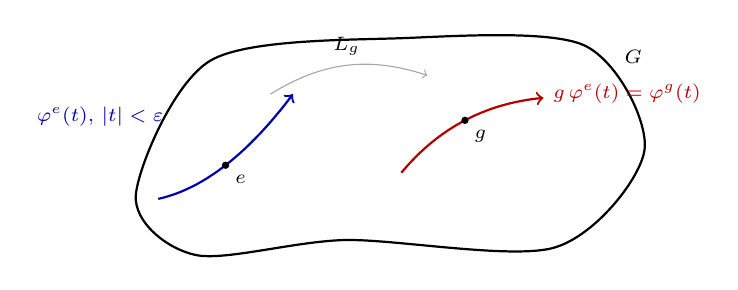
\begin{tikzpicture}[scale=0.95]
\draw[thick] plot[smooth cycle] coordinates {(-3.4,-0.6) (-2.4,1.2) (0.2,1.5) (2.6,1.4) (3.4,0.0) (2.2,-1.3) (-0.6,-1.2) (-2.6,-1.4)};
\node[font=\scriptsize] at (3.25,1.25) {$G$};
\draw[blue!70!black, thick, ->] plot[smooth] coordinates {(-3.100,-0.650) (-3.054,-0.639) (-3.008,-0.627) (-2.962,-0.613) (-2.915,-0.598) (-2.869,-0.582) (-2.823,-0.565) (-2.777,-0.546) (-2.731,-0.526) (-2.685,-0.504) (-2.638,-0.482) (-2.592,-0.458) (-2.546,-0.432) (-2.500,-0.406) (-2.454,-0.378) (-2.408,-0.348) (-2.362,-0.318) (-2.315,-0.286) (-2.269,-0.252) (-2.223,-0.218) (-2.177,-0.182) (-2.131,-0.145) (-2.085,-0.106) (-2.038,-0.066) (-1.992,-0.025) (-1.946,0.017) (-1.900,0.061) (-1.854,0.106) (-1.808,0.153) (-1.762,0.200) (-1.715,0.249) (-1.669,0.300) (-1.623,0.351) (-1.577,0.404) (-1.531,0.459) (-1.485,0.514) (-1.438,0.571) (-1.392,0.630) (-1.346,0.689) (-1.300,0.750)};
\draw[red!70!black, thick, ->] plot[smooth] coordinates {(0.150,-0.300) (0.189,-0.254) (0.228,-0.210) (0.268,-0.166) (0.308,-0.124) (0.349,-0.082) (0.390,-0.042) (0.432,-0.003) (0.475,0.036) (0.517,0.073) (0.561,0.109) (0.605,0.144) (0.649,0.178) (0.694,0.211) (0.740,0.243) (0.786,0.274) (0.833,0.304) (0.880,0.333) (0.928,0.360) (0.976,0.387) (1.024,0.413) (1.074,0.437) (1.123,0.461) (1.174,0.483) (1.225,0.505) (1.276,0.525) (1.328,0.544) (1.380,0.563) (1.433,0.580) (1.487,0.596) (1.541,0.611) (1.595,0.625) (1.650,0.638) (1.706,0.650) (1.762,0.661) (1.818,0.671) (1.875,0.680) (1.933,0.688) (1.991,0.694) (2.050,0.700)};
\fill (-2.2,-0.2) circle (1.4pt) node[below right, font=\scriptsize] {$e$};
\fill (1.0,0.4) circle (1.4pt) node[below right, font=\scriptsize] {$g$};
\draw[->, gray!70, bend left=25] (-1.6,0.75) to node[above, font=\scriptsize, text=black] {$L_g$} (0.5,1.0);
\node[blue!70!black, font=\scriptsize, anchor=east] at (-2.9,0.45) {$\varphi^e(t)$, $|t| < \varepsilon$};
\node[red!70!black, font=\scriptsize, anchor=west] at (2.05,0.75) {$g\,\varphi^e(t) = \varphi^g(t)$};
\end{tikzpicture}
